\documentclass[12pt,brazil]{book}
\usepackage{babel}
\usepackage[utf8x]{inputenc}
\usepackage[top=2.5cm,left=2.5cm,bottom=2.5cm,right=2.5cm]{geometry}
\usepackage{url}
\usepackage{graphicx}
\usepackage{html}

\newcommand{\sep}{$\rightarrow$}

\title{Genoslab Handbook}
\author{Pedro Kröger}

\begin{document}
\graphicspath{{figs/}}

\maketitle

\begin{htmlonly}
  Baixe a versão em pdf \htmladdnormallink{aqui}
  {http://genos.mus.br/handbook/genoslab-handbook.pdf}.
\end{htmlonly}

\tableofcontents

\part{Introdução}
\label{part:introducao}

% TODO
% \chapter{Como contribuir para esse documento}
% \label{sec:como-contribuir-para}

\part{Ferramentas}
\label{part:ferramentas}

\chapter{Repositórios debian}
\label{cha:repositorios-debian}

Para instalar o csound5 você deve usar o pacote debian do Genos. Para
isso coloque a seguinte linha no seu \texttt{/etc/apt/sources.list}
(como root):

\begin{verbatim}
deb http://genos.mus.br/ debian/
\end{verbatim}

Em seguida rode o comando

\begin{verbatim}
aptitude update
\end{verbatim}

Agora você pode instalar os programas disponíveis no genos digitando
algo como o comando abaixo como root.

\begin{verbatim}
aptitude install <nome do programa>
\end{verbatim}

\section{Debian}
\label{sec:debian}

\section{Modo emacs para apt}
\label{sec:modo-emacs-para}

http://www.netfort.gr.jp/~dancer/software/apt-mode.html

\chapter{Git}
\label{cha:git}

\section{Introdução}
\label{sec:introducao}

O Git (o ``g'' é pronunciado como na palavra gato e não como ``jit'')
é um programa para controle de versão distribuído desenvolvido por
Linus Torvalds (o criador do Linux) e mantido por Junio C Hamano. A
página do git em \url{http://git.or.cz/} tem vários tutoriais e
manuais.

\section{Instalação}
\label{sec:instalacao-3}

Para instalar o git no debian execute o seguinte comando.

\begin{verbatim}
aptitude install git-core git-completion git-doc git-gui gitk ssh
\end{verbatim}

É uma boa idéia configurar o git para usar o seu nome e email:

\begin{verbatim}
git config --global user.name "Seu Nome"
git config --global user.email "seu@email.com.br"
\end{verbatim}

\section{Repositórios do genos}
\label{sec:acesso-de-escrita}

O genos mantém diversos repositórios listados em
\url{git.genos.mus.br}. Para ter acesso de escrita você precisa criar
uma chave pública de criptografia. Para isso rode o comando:

\begin{verbatim}
ssh-keygen -t rsa
\end{verbatim}

Esse comando vai fazer uma série de perguntas como o tamanho da chave,
seu nome e email, etc. Se você não souber a resposta para alguma
pergunta não precisa se preocupar, o valor padrão deve ser o
suficiente. Quando ele pedir uma passphrase, certifique-se que você
não vai esquecê-la! A chave pública vai ser geradad no arquivo
\texttt{~/.ssh/id\_rsa.pub}. Para ter acesso de escrita nos
repositórios do genos envie o arquivo para Pedro Kroger.

Se você enviou a chave pública e seu acesso foi liberado, você pode
baixar um projeto no repositório do genos com o comando abaixo:

\begin{verbatim}
git clone ssh://cons@genos.mus.br/repos/<nome do projeto>
\end{verbatim}

Por exemplo, para baixar o projeto analise-harmonica você deve
digitar:

\begin{verbatim}
git clone ssh://cons@genos.mus.br/repos/analise-harmonica.git
\end{verbatim}

Contudo, se você não tem acesso de escrita ao repositório, ou seja,
não tem permissão para modificar o repositório diretamente, você ainda
pode baixar um projeto e contribuir mudanças (veja a seção
\ref{sec:enviando-patches}). Para isso baixe o repositório com o
comando abaixo:

\begin{verbatim}
git clone http://genos.mus.br/repos/<nome de repositório>
\end{verbatim}

\section{Comandos básicos}
\label{sec:comandos-basicos}

Você deve gravar suas mudanças com

\begin{verbatim}
git commit -m "mensagem descrevendo o commit"
\end{verbatim}

Use o comando abaixo para enviar suas mudanças para o repositório
central:

\begin{verbatim}
git push
\end{verbatim}

Para atualizar sua cópia local, ou seja, para baixar as mudanças que
outros tenham feito no repositório, use os comandos:

\begin{verbatim}
git fetch
git rebase origin/<branch remoto>
\end{verbatim}

onde <branch remoto> é o branch remoto onde o desenvolvimento
acontece. Provavelmente é master.

Para reverter as mudanças que não foram enviadas use

\begin{verbatim}
git checkout -f
\end{verbatim}


\section{Pull vs Rebase}

Existem dois jeitos de importar as mudanças de um repositório remoto
pro repositório local. Elas são o ``pull'' e o ``rebase''. A diferença
é a forma como as mudanças locais são mantidas na hora de importar as
remotas.

Imagine uma árvore de commits assim (onde local é o branch atual de desenvolvimento):

\begin{verbatim}
                     A---B---C local
                    /
               D---E---F---G master
\end{verbatim}

Após um ``git pull'' aplicado no computador local, a árvore fica:

\begin{verbatim}
                     A---B---C---F'--G' local
                    /           /
               D---E---F---G ----master
\end{verbatim}

Após um git push, a árvore no repositório remoto fica

\begin{verbatim}
                     A---B---C---F'--G'-- 
                    /           /        \
               D---E---F---G -------------A'--B'--C'--F''--G''  master
\end{verbatim}

Isso não é muito interessante por serem feitos, ao todo, dois merges
das mudanças locais no repositório remoto. Com mais de duas pessoas
fazendo mudanças ao mesmo tempo esse método gera árvores de histórico
complicadas e difíceis de entender depois, com vários merges.

Uma alternativa é usar ``git rebase origin/master'' em vez de ``git
pull''. Fazendo isso, a árvore local, que era

\begin{verbatim}
                     A---B---C local
                    /
               D---E---F---G master
\end{verbatim}

fica

\begin{verbatim}
                             A'---B'---C' local
                            /
               D---E---F---G master
\end{verbatim}

Após um ``git push'', a árvore do servidor fica

\begin{verbatim}
                             A'---B'---C'-
                            /             \
               D---E---F---G ---------------  master
\end{verbatim}

ou

\begin{verbatim}
               D---E---F---G---A'--B'--C'-----  master
\end{verbatim}

o que é muito mais limpo. Mesmo com várias pessoas desenvolvendo isso
tende a gerar históricos mais lineares.

\section{Escrevendo boas mensagens de commit}
\label{sec:escr-boas-mens}

Além de usar a opção \texttt{-m} para indicar a mensagem de commit,
você também pode digitar apenas \texttt{git commit} onde o git vai
abrir o editor padrão para você digitar a mensagem de commit. Em geral
o editor padrão é o vi. Eu sugiro que você coloque a linha abaixo no
seu \texttt{~/.bashrc}:

\begin{verbatim}
  export EDITOR="emacs"
\end{verbatim}

Desse modo o git sempre vai abrir o emacs para pedir a mensagem de
commit.

Em geral uma mensagem de commit tem o seguinte formato:

\begin{verbatim}
primeira linha

texto mais longo texto mais longo texto mais longo
texto mais longo texto mais longo texto mais longo
texto mais longo texto mais longo texto mais longo 
\end{verbatim}

Onde a primeira linha é um breve sumário da modificações, o texto mais
longo contém mais detalhes. Observe que elas são separadas por uma
linha em branco.

\section{Usando diferentes ramos}
\label{sec:usando-o-git}

Para ver os ramos do repositório basta usar o comando

\begin{verbatim}
git branch
\end{verbatim}

Para mudar de ramo usa-se o comando

\begin{verbatim}
git checkout
\end{verbatim}

Mudando do ramo master para novo-ramo:

\begin{verbatim}
git checkout novo-ramo
\end{verbatim}

Conferindo o novo ramo:

\begin{verbatim}
git branch
  master
* novo-ramo
\end{verbatim}

Para criar um novo ramo e mudar para ele automaticamente usa-se

\begin{verbatim}
git checkout -b novo-ramo
\end{verbatim}

Para ver a lista de commits no novo-ramo em relação a master (pode-se
usar a opção \texttt{-p} para ver um diff do código:

\begin{verbatim}
git log  master..novo-ramo
\end{verbatim}

Para enviar um novo ramo para o repositório remoto:

\begin{verbatim}
git push origin ramo-local:ramo-remoto
\end{verbatim}

Talvez você tenha que usar o caminho completo para o ramo, como em:

\begin{verbatim}
git push origin refs/heads/ramo-local:refs/heads/ramo-remoto
\end{verbatim}

Para listar os ramos em um repositório remoto

\begin{verbatim}
git branch -r
\end{verbatim}

Para baixar um ramo no repositório remoto usa-se \texttt{git branch}
com a opção \texttt{--track}, indicando qual o nome do ramo local e o
nome do ramo remoto. É uma boa prática ter o mesmo nome para os ramos
local e remoto.

\begin{verbatim}
git branch --track novo-ramo origin/novo-ramo
\end{verbatim}

O nome \texttt{origin} nada mais é que um alias para a localização de
um repositório. Essa informação fica armazenada no arquivo
\texttt{.git/config} dentro do repositório. O trecho do
\texttt{.git/config} referente a configuração de \texttt{origin} pode
ser vista abaixo:

\begin{verbatim}
[remote "origin"]
        url = ssh://cons@genos.mus.br/repos/teste.git
        fetch = +refs/heads/*:refs/remotes/origin/*
\end{verbatim}

Veja na seção \ref{sec:o-arquivo-config} outras possibilidades de uso
para o arquivo \texttt{.git/config}.

Para manter os ramos atualizados, \texttt{git pull} e \texttt{git
  push} devem ser suficientes. O Git mantém cada ramo separado sem
interferir no outro. Contudo, mudanças sem commit vão aparecer em
todos os ramos.

Para mesclar as mudanças do branch \texttt{master} no seu ramo é só
fazer:

\begin{verbatim}
git pull .
\end{verbatim}

\section{Escolhendo commits específicos (cherry picking)}
\label{sec:escolh-comm-espec}

Você pode aplicar um commit específico na sua árvore com
\texttt{cherry-pick}. No exemplo abaixo estamos no branch master e o
commit 85cd08ee1aec0fbd3cf3d696a70872639e59212f aconteceu no branch
novo-ramo. Ele vai aplicar apenas esse commit em master.

\begin{verbatim}
git cherry-pick 85cd08ee1aec0fbd3cf3d696a70872639e59212f
\end{verbatim}

Isso é útil quando você corrigiu um bug em um ramo de desenvolvimento
e quer replica-lo no ramo principal.

\section{Resolvendo conflitos}
\label{sec:resolvendo-conflitos}

Quando um merge não é resolvido automaticamente pelo git ele indica
isso claramente. Você não vai conseguir dar um commit. Tanto commit
quanto status vão mostrar os arquivos que precisam resolver os
conflitos:

\begin{verbatim}
git commit
file.txt: needs merge
\end{verbatim}

Git vai marcar os conflitos no arquivo usando marcadores de conflito.
Abaixo podemos ver um conflito marcado com duas versões:

\begin{verbatim}
<<<<<<< HEAD:file.txt
Uma versão
=======
Outra versão
>>>>>>> 77976da35a11db4580b80ae27e8d65caf5208086:file.txt
\end{verbatim}

Tudo que você precisa fazer é editar o arquivo para resolver os
conflitos e dar um commit com:

\begin{verbatim}
git add file.txt
git commit
\end{verbatim}

Se você usa emacs pode usar o \texttt{M-x vc-resolve-conflicts} para
lhe auxiliar na resolução de conflitos (ele funciona como o ediff).

\section{Revisões antigas}
\label{sec:revisoes-antigas}

Você pode ver uma versão antiga de um arquivo com \texttt{cat-file}:

\begin{verbatim}
git cat-file -p tags/v1.4.3:git.c
git cat-file -p f5f75c652b9c2347522159a87297820103e593e4:git.c
\end{verbatim}

\section{Enviando patches}
\label{sec:enviando-patches}

Para criar patches com suas modificações você deve usar o
\texttt{format-patch}. Esse comando vai gerar uma série de arquivos
numerados, como \texttt{0001-mais-stuff.patch}. Você deve enviar esses
arquivos para a lista de discussão apropriada.

\begin{verbatim}
 git format-patch origin
\end{verbatim}

Se a quantidade de patches for muito grande, você pode usar o
\texttt{git-send-email}, caso contrário é ok usar seu cliente de email
favorito.

\section{Configuração}
\label{sec:configuracao}

\subsection{Usando abreviações}
\label{sec:usando-abreviacoes}

Eu sugiro que você coloque algo como a linha abaixo no seu
\texttt{~/.bashrc}.

\begin{verbatim}
export repos=ssh://cons@genos.mus.br/repos
\end{verbatim}

Desse modo você poderá baixar um projeto de uma maneira mais fácil:

\begin{verbatim}
git clone $repos/analise-harmonica.git
\end{verbatim}

\subsection{O arquivo config}
\label{sec:o-arquivo-config}

Você pode configurar o arquivo \texttt{.git/config} de um repositório
local para usar nomes abreviados. Isso é particularmente útil se está
usando mais de um repositório ou ramos diferentes.

\begin{verbatim}
cat >>.git/config <<EOF
[remote "public-repo"]
        url = ssh://yourserver.com/~you/proj.git
EOF
\end{verbatim}

Você pode fazer a mesma coisa com \texttt{git remote}:

\begin{verbatim}
git remote add public-repo ssh://example.com/project.git
\end{verbatim}

\subsection{Saída colorida}
\label{sec:saida-colorida}

Se você é viciado em saída colorida vai querer executar os comandos abaixo:

\begin{verbatim}
git config --global color.diff auto
git config --global color.status auto
git config --global color.branch auto
\end{verbatim}

\chapter{Gravação de CD e DVD}
\label{cha:gravacao-de-cd}

\section{Copiando um CD ou DVD}
\label{sec:copiando-um-cd}

A maneira mais fácil de copiar um DVD ou CD completamente é usando o
\texttt{dd}. A opção \texttt{if} (\textit{input file}) indica o
dispositivo do DVD ou CD e a opção \texttt{of} (\texttt{output file})
indica o nome da imagem que será gerada:

\begin{verbatim}
dd if=/dev/sr1 of=arquivo.iso
\end{verbatim}

O arquivo gerado será uma réplica exata do CD. Inclusive você pode
montar a imagem usando mount:

\begin{verbatim}
mount -o loop /tmp/arquivo.iso /mnt
\end{verbatim}

\section{Identificando o fabricante da mídia}
\label{sec:ident-o-fabr}

Para identificar o verdadeiro fabricante de uma mídia de DVD use o
comando \texttt{dvd+rw-mediainfo} como abaixo:

\begin{verbatim}
dvd+rw-mediainfo /dev/dvd
\end{verbatim}

Para identificar o verdadeiro fabricante de uma mídia de CD use a
opção \texttt{-atip} do wodim.

\begin{verbatim}
wodim -atip 
\end{verbatim}

\section{Recuperando dados}
\label{sec:recuperando-dados}

Se o disco tem problemas o \texttt{ddrescue} pode ser uma boa opção.
Para ler um disco:

\begin{verbatim}
ddrescue /dev/dvd DVD.iso DVD.log
\end{verbatim}

Se \texttt{ddrescue} reportar algum erro, tente uma segunda vez com o
acesso direto ao disco ativado:

\begin{verbatim}
ddrescue -d -r1 /dev/dvd DVD.iso DVD.log
\end{verbatim}

\chapter{BibTeX}
\label{cha:bibtex}

\section{Introdução}
\label{sec:introducao-1}

BibTeX é um formato de arquivo para citações bibliográficas.

\section{Utilitários para o BibTeX}
\label{sec:utilitarios-para-o}

Os artigos \textit{Bibliography prettyprinting and syntax checking} e
\textit{A Bibliographer's Toolbox} de Nelson H. F. Beebe contém
informações importantes sobre ferramentas para lidar com o BibTeX.
Eles podem ser baixados em
\url{http://www.math.utah.edu/~beebe/publications/1993/tugboat-14-4-395-dec-1993.pdf}
 e \url{http://www.math.utah.edu/~beebe/talks/2004/pt2004/pt2004.pdf},
respectivamente. A página \textit{Manipulating BibTeX Bibliographies}
em \url{http://liinwww.ira.uka.de/bibliography/Bib.Format.html} também
contém informações importantes.

http://ebib.sourceforge.net/

utilitários para emacs

http://www.math.utah.edu/pub/emacs/

\section{Citando publicações on-line}
\label{sec:citando-publ-line}

As urls para documentos devem ser colocadas no campo ``url''. Se
existem mais de uma url separe-as com espaços em branco ou use vários
campos na forma ``xxx-url'' onde xxx é algum texto explicativo como
dvi, pdf etc. Urls de resumos devem ser colocadas no campo
``abstract-url''. Os estilos is-{abbrv,alpha,plain,unsrt} reconhecem
os campos ISBN, URL, IOB, dentre outros.

\begin{verbatim}
abntex - LaTeX class for writing documents in ABNT standard
bibclean - pretty-printer for BibTeX databases
bibcursed - An interactive program to edit BibTeX bibliographies
bibindex - Fast lookup in BibTeX bibliography data bases
bibtex2html - filters BibTeX files and translates them to HTML
bibtool - tool for BibTeX database manipulation
gbib - user-friendly editor and browser for BibTeX databases
jed - editor for programmers (textmode version)
kbibtex - BibTeX editor for KDE
pybliographer - tool for manipulating bibliographic databases
search-ccsb - BibTeX search tool
search-citeseer - BibTeX search tool
tellico - collection manager for books, videos, music
tellico-data - collection manager for books, videos, music [data]
\end{verbatim}

% \section{Dicas gerais}
% \label{sec:dicas-gerais}

% Não use et al.

% busca de bibtex na internet  +@Book +Knuth

% ``A colleague once quipped: “When you see a paper cited as
% Jones et al., it means that Jones got the credit, but Al did the
% work.”''

% Karlsruhe Bibliography Archive

% considerar campo bibdate

% aprender teclas de atalho bibtex

% fazer scripts para converter dados de webpage para gerar bibtex

% usar full journal names

% usar strings para abreviar

% Two programs, journal.awk and publisher.awk, filter an input BIBTEX
% stream, and output a new stream in which journal, publisher, and
% address values that have been found to match any of several common
% variations are replaced by the standardized abbreviations, and the
% data stream is prefixed by corresponding @String{. . . } definitions.

% %% proteção de titulos

% The easy cases are those words with mixed case, such as BiCGS and
% McLeod, which are always known to be proper nouns in need of
% protection;

% %% dividir arquivos bibtex
% The bibsplit21 tool splits them into parts, separating entries into
% different output files according to one of several criteria: author,
% citation label, citation count, or year range. I’ve had to do this
% numerous times with journalspecific bibliographies as their entry
% count grows. Usually, subdivision into decade-specific bibliographies
% suffices.

% % agrep

% mostra aproximações (com erros), mostra paragrafo inteiro (entrada
% completa do bibtex)

% bibsearch

% aspell para bibtex com arquivos de exceção

% chkdelim

% Doubled words Doubled-word errors (as in the the book) are difficult
% for humans to spot. My dw program (http://www.math.utah.edu/pub/dw/)

% bibparse31
% • biblex (included with bibparse)
% • bibunlex (included with bibparse)
% • bibclean32

% The first of these, bibparse, merely confirms that its input conforms
% to the grammar: a successful validation produces no output. I use this
% as an initial check of updates to the bibliographic archives before
% even attempting to run LATEX and BIBTEX: any error from bibparse
% immediately aborts the entire automated installation process.

% The second, biblex, parses the input and produces a token stream that
% is much easier to handle by other tools.

% The third, bibunlex, reassembles a biblex token stream, possibly after
% filtering, reconstructing a valid BIBTEX file.

% The fourth, and most powerful, bibclean, has been of enormous
% importance in my bibliographic work. It is based on the same rigorous
% grammar as bibparse, but is implemented completely independently with
% a carefully-hand-coded parser, instead of the machine-generated parser
% in bibparse. That way, there are two independent checks on the
% validity of the syntax of BIBTEX data. bibclean normally produces a
% prettyprinted bibliography file in which numerous repairs and checks
% have been made on the data. For hundreds of thousands of examples, see
% the TEX Users Group Bibliography Archive33 and the BibNet Project
% archive.34 On request, however, bibclean produces the same token
% streams as biblex.

% validação de field: bibclean e bibcheck

% • biblabel36 and its companion tool citesub, and an independent
% implementation in the emacs BIBTEX-LABELS37 library, generate
% standardized citation labels that are unlikely to conflict with those
% of other entries, and importantly, that are easy for humans to predict
% as well.

% • bibsort38 sorts entries in a bibliography by any of a half-dozen
% different criteria.

% • biborder39 reorders fields within a BIBTEX entry into a standard
% order, making the entries much easier to read.

% • bibjoin40 merges adjacent BIBTEX entries that appear to describe the
% same publication, discarding duplicate data, choosing more detailed
% values over less detailed ones (e.g., in the author field, the longer
% of Donald E. Knuth and D. E. Knuth), and otherwise leaving the
% duplicate fields adjacent for manual correction.

% • bibdup41 checks for duplicate abbreviations and entries.

% • For interactive location and repair of problems, the emacs function
% find-duplicate-label from the BIBTOOLS library42 finds the next
% occurrence of consecutive entries with the same citation label. The
% function find-duplicate-key from the same library finds the next
% instance of duplicate adjacent field names in a single BIBTEX entry.

\chapter{SLIME}
\label{cha:slime}


\part{Programas de áudio}
\label{part:programas-de-audio}

\chapter{CLM---Common Lisp Music}
\label{cha:clm-common-lisp}

\section{Pré-requisitos}
\label{sec:pre-requisitos}

Para compilar o CLM você precisará do gcc (o compilador C do projeto
GNU) e outras ferramentas instaladas. Além disso, o CLM não é um
programa auto-contido como o Csound. Ele é na verdade uma biblioteca
de funções Lisp. Para utiliza-lo você precisará de um compilador Lisp.
Eu recomendo o SBCL. Finalmente, você precisará de um bom editor. Eu
recomendo o Emacs com o Slime. O comando abaixo deve instalar tudo que
você precisa para começar:

\begin{verbatim}
aptitude install gcc emacs22 slime sbcl csh
\end{verbatim}

\section{Instalação}
\label{sec:instalacao}

Infelizmente não existe um pacote do CLM para o debian, então teremos
que instala-lo manualmente. Além disso, vamos instalar de uma maneira
que é mais fácil mas não é necessariamente robusta. Contudo essa
maneira é suficiente para você iniciar no programa. No futuro veremos
maneiras mais robustas de instalar o CLM.

Baixe a última versão do CLM no site do projeto em
\url{http://ccrma.stanford.edu/software/clm/} e descompacte o tar.gz
em um diretório. O diretório clm-3 será criado quando o arquivo for
descompactado. Os comandos abaixo efetuam essas operações:

\begin{verbatim}
wget ftp://ccrma-ftp.stanford.edu/pub/Lisp/clm-3.tar.gz
tar -xzf clm-3.tar.gz
\end{verbatim}

Em seguida coloque o seguinte código no final do arquivo
\verb|~/.swank.lisp|:

\begin{verbatim}
(defun clm ()
  (require :asdf)
  (setf *clm-dir* #p"/home/kroger/clm-3/")
  (push *clm-dir* asdf:*central-registry*)
  (asdf:operate 'asdf:load-source-op :clm)
  (setf *default-pathname-defaults* *clm-dir*))
\end{verbatim}

Observe que dentro do diretório clm-3 existem diversos arquivos. Os
arquivos com a extensão *.ins definem instrumentos do CLM e são os que
nos interessam. 

Para iniciar o CLM abra o emacs e slime com \texttt{M-x slime}. O REPL
(\textit{Read Eval Print Loop}) é o modo interativo de Lisp. Nele você
pode digitar expressões e obter resultados. Para programas maiores é
desconfortável entrar expressões no REPL, mas para testar coisas ele é
bastante útil. No REPL digite o comando abaixo para iniciar o CLM:

\begin{verbatim}
(clm)
\end{verbatim}

Sempre que você quiser usar o CLM basta iniciar o emacs, carregar o
slime e digitar ``(clm)'' no REPL.

Se você quiser iniciar o slime com uma tecla de atalho, coloque a
linha abaixo no seu \texttt{.emacs}:

\begin{verbatim}
(global-set-key [f9] 'slime)
\end{verbatim}

\section{Uso básico}
\label{sec:uso-basico}

Tendo compilado o CLM você pode carregar e usar instrumentos definidos
nos arquivos *.ins. Por exemplo, o arquivo v.ins define um instrumento
de nome ``fm-violin'' que sintetiza um violino usando FM. Você pode
carregar um instrumento com o comando abaixo:

\begin{verbatim}
(load "v")
\end{verbatim}

Finalmente, você pode usar o instrumento com o comando abaixo:

\begin{verbatim}
(with-sound () (fm-violin 0 1 440 .1)) 
\end{verbatim}

\section{Para saber mais}
\label{sec:para-saber-mais}

Para saber mais sobre a instalação do CLM veja o arquivo README.clm.
O manual está no arquivo clm.html. Ambos estão no diretório do CLM.

\chapter{Nyquist}
\label{cha:nyquist}

\section{Instalação}
\label{sec:instalacao-1}

Para instalar o nyquist é só usar o aptitude:

\begin{verbatim}
aptitude install nyquist
\end{verbatim}

O binário do nyquist se chama \texttt{ny}. Se você digitar \texttt{ny}
no terminal um prompt interativo vai abrir e esperar por comandos.
Você pode digitar algo simples para testar se o programa está
funcionando. O comando abaixo vai tocar um dó central:

\begin{verbatim}
(play (osc 60))
\end{verbatim}

\begin{htmlonly}
  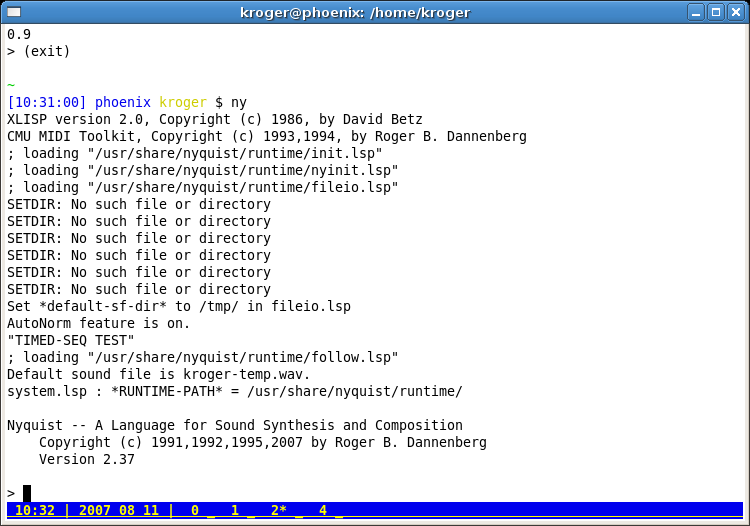
\includegraphics{ny1}
\end{htmlonly}

\begin{latexonly}
  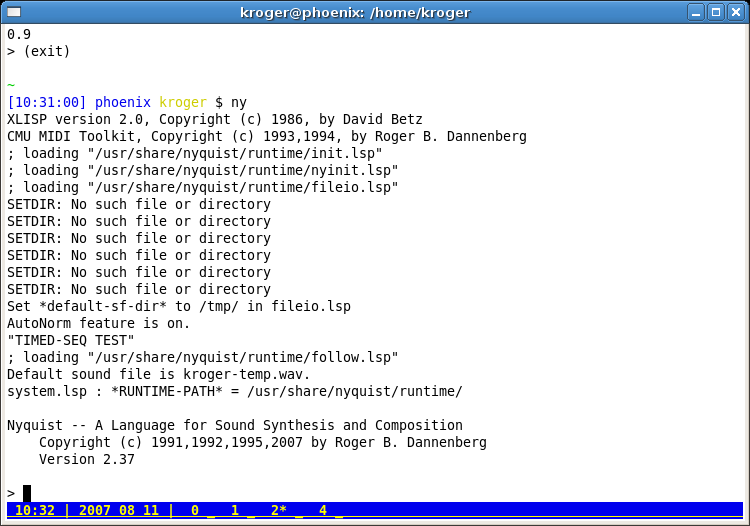
\includegraphics[scale=.5]{ny1}
\end{latexonly}

O manual do nyquist está disponível em
\url{http://www.cs.cmu.edu/~rbd/doc/nyquist/root.html} e em
\url{/usr/share/doc/nyquist/doc/home.html} se você instalou o pacote
debian.

\section{O modo para emacs}
\label{sec:o-modo-para-2}

Um modo preliminar do emacs para o nyquist pode ser encontrado em
\url{http://www.genos.mus.br/handbook/src/inf-nyquist.el}. Baixe o arquivo em
algum lugar no seu computador (eu sugiro \verb|~/lib/emacs/|) e
coloque as seguintes linhas no seu \texttt{.emacs}:

\begin{verbatim}
(autoload 'run-nyquist-lisp   "inf-snd" "Start inferior Snd-Lisp process" t)
(autoload 'nyquist-lisp-mode  "inf-nyquist" "Load nyquist-lisp-mode." t)
(setq inf-nyquist-lisp-program-name "ny")

(add-to-list 'auto-mode-alist '("\\.ny$" . nyquist-lisp-mode))

(add-hook 'nyquist-lisp-mode-hook
          (lambda ()
            (slime-mode nil)
            (local-set-key "\r" 'newline-and-indent)
            (setq lisp-indent-function 'common-lisp-indent-function)
            (setq indent-tabs-mode nil)))
\end{verbatim}

Todos os arquivos com a extensão \texttt{.ny} estarão associados ao
nyquist.

\section{Usando o nyquist com o emacs}
\label{sec:usando-o-nyquist}

Inicie o emacs e abra um arquivo com a extensão \texttt{.ny}, por
exemplo, \texttt{foo.ny}. Observe que o item ``Nyquist'' vai aparecer
no menu. Para iniciar o nyquist escolha no menu Nyquist\sep Start
Nyquist-lisp process ou \texttt{C-c C-s} no teclado. Um buffer chamado
\texttt{*Nyquist-lisp*} será aberto. Esse buffer é o modo interativo
do nyquist.

Você pode digitar comandos do nyquist no arquivo aberto (no nosso caso
\texttt{foo.ny}) e enviá-los para o nyquist com \texttt{C-x C-e} ou
através do menu em Nyquist\sep Send last Sexp.

\begin{htmlonly}
  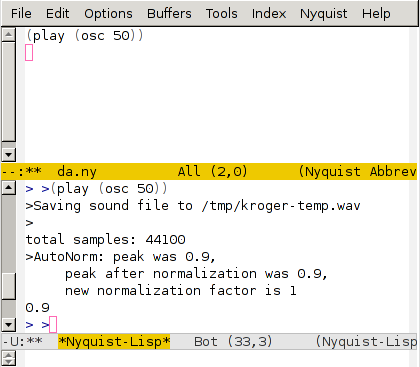
\includegraphics{ny2}
\end{htmlonly}

\begin{latexonly}
  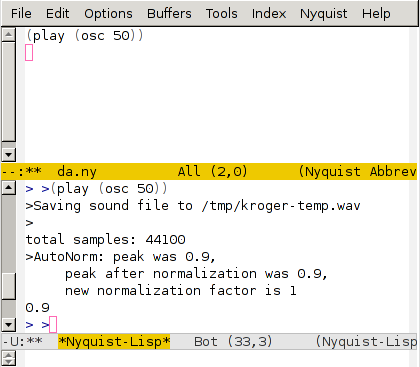
\includegraphics[scale=.5]{ny2}
\end{latexonly}

\section{Desenvolvendo plugins do audacity com o nyquist}
\label{sec:desenv-plug-do}

O audacity tem uma versão do nyquist embutida, de modo que plugins
podem ser desenvolvidos com ele. Os arquivos de plugins devem ser
colocados em \texttt{~/.audacity-files/plug-ins} e o audacity deve ser
reiniciado toda vez que um novo plugin for criado. 

Crie um arquivo \texttt{teste.ny} com o seguinte conteúdo:

\begin{verbatim}
;nyquist plug-in
;version 1
;type process
;name "Teste de fade in"
;action "Fading In..."
(mult (ramp) s)
\end{verbatim}

Observe que o efeito ``Teste de fade in'' vai aparecer no menu de
efeitos do audacity.

Um breve tutorial de como criar plugins do audacity com o nyquist pode
ser visto em \url{http://audacity.sourceforge.net/help/nyquist3}.

\chapter{SuperCollider}
\label{cha:supercollider}

O SuperCollider é uma linguagem de programação para síntese de áudio
em tempo real e composição algorítmica. A página do programa fica em
\url{http://supercollider.sourceforge.net}.

\section{Instalação}
\label{sec:instalacao-2}

Para instalar o supercollider no debian é só executar o comando
abaixo:

\begin{verbatim}
aptitude install supercollider supercollider-doc supercollider-server
\end{verbatim}

\section{Uso básico}
\label{sec:uso-basico-1}

Nós vamos usar o SuperCollider dentro do Emacs. Para ativar o modo
sclang que permite interagir com o SC coloque a seguinte linha no seu
\texttt{~/.emacs}:

\begin{verbatim}
(require 'sclang)
\end{verbatim}

O SuperCollider usar o jack para entrada e saida, então tenha certeza
de te-lo rodando antes de carregar o SC. Inicie o emacs e carregue o
modo sclang:

\begin{verbatim}
M-x sclang-start
\end{verbatim}

O emacs vai abrir dois \textit{buffers}, um chamado *SCLang:Workspace*
e outro *SCLang:PostBuffer*. No Workspace você pode digitar comandos
do SC. Os resultados dos comandos vão aparecer no PostBuffer.

O menu SCLang no emacs tem diversos comandos para lidar com o SC. O
mais importante é como parar um som que esteja tocando. Você pode
acessá-lo em SCLang$\leftarrow$Stop Main no menu, ou pelo teclado com
\texttt{C-c C-s}. Para computar uma linha de código use \texttt{C-c
  C-c } (ou \textit{Evaluate Line} no menu).

Para iniciar o servidor, digite a linha abaixo e, com o cursor em
qualquer lugar da linha, digite \texttt{C-c C-c}:

\begin{verbatim}
s = Server.local.boot;
\end{verbatim}

Agora compute a linha abaixo para tocar um lá continuamente (lembre de
usar o \texttt{C-c C-s} para parar o som).

\begin{verbatim}
{SinOsc.ar(442, 0, 0.2) }.play;
\end{verbatim}

Finalmente, para demonstrar o poder expressivo do SuperCollider, veja
o que é possível de fazer com uma única linha de código:

\begin{verbatim}
play{SinOsc.ar(OnePole.ar(Mix(LFSaw.ar([1,0.99],[0,0.6],2000,2000).trunc([400,600])*[1,-1]),0.98)).dup*0.1};
\end{verbatim}

\section{Para saber mais}
\label{sec:para-saber-mais-1}

O site do SuperCollider tem vários tutoriais na página
\url{http://supercollider.sourceforge.net/learning}.

\chapter{Csound}
\label{cha:csound}

\section{Instalação}
\label{sec:instalacao-4}

Para instalar o csound5 você deve usar o pacote debian do Genos. Veja
a seção \ref{cha:repositorios-debian} para ver como configurar seu
computador para usar o repositório de pacotes do Genos.

Tendo configurado o repositório do genos é só dar o comando abaixo
para instalar o csound.

\begin{verbatim}
aptitude install csound5
\end{verbatim}

Finalmente coloque a linha abaixo no seu \texttt{.bashrc}:

\begin{verbatim}
export OPCODEDIR=/usr/lib/csound/plugins
\end{verbatim}

\section{Uso básico}
\label{sec:uso-basico-2}

Para testar a instalação, crie um arquivo \texttt{teste.orc} com o seguinte
conteúdo:

\begin{verbatim}
instr 1
  a1        oscil     1000,440,1
            out       a1       
endin
\end{verbatim}

Crie também um arquivo \texttt{teste.sco} com o conteúdo abaixo:

\begin{verbatim}
f1  0 1024  10    1

i1 0 3
\end{verbatim}

Para usar o csound no terminal basta digitar \texttt{csound
  <orquestra> <partitura>}, por exemplo:

\begin{verbatim}
csound teste.orc teste.sco
\end{verbatim}

O csound vai gerar um arquivo de áudio chamado \texttt{teste.wav}.
Para ouvir em tempo real use a opção \texttt{-o}:

\begin{verbatim}
csound -odac teste.orc teste.sco
\end{verbatim}

Essa opção também pode ser usada para determinar o nome do arquivo de
áudio da saída:

\begin{verbatim}
csound -o teste.wav teste.orc teste.sco
\end{verbatim}

\section{O modo para emacs}
\label{sec:o-modo-para}

Um modo avançado e completo do csound para emacs está disponível em
\url{www.zogotounga.net/comp/csoundx.html}. Execute o comando abaixo
para baixar e descompactar o arquivo:

\begin{verbatim}
http://www.zogotounga.net/comp/stef-elisp-2.09.zip
unzip stef-elisp-2.09.zip
\end{verbatim}

Em seguida coloque as seguintes linhas no seu \texttt{.emacs}. Não
esqueça de trocar o diretório do comando \texttt{add-to-list} para o
diretório onde você baixou o modo.

\begin{verbatim}
(add-to-list 'load-path "/home/kroger/lib/emacs/stef-elisp/")
(require 'stef-elisp)
\end{verbatim}

A medida que você for customizando seu emacs, pode querer colocar
todas as extensões em um diretório específico. Eu sugiro
\verb|~/lib/emacs|.

\chapter{Snd}
\label{cha:snd}

\section{Instalação}
\label{sec:instalacao-5}

Para instalar a versão mais nova do snd configure seu computador para
usar o repositório de pacotes debian do genos. Veja como fazer isso na
seção \ref{cha:repositorios-debian}. Para instalar o snd é só digitar
o comando abaixo (como root):

\begin{verbatim}
aptitude install snd
\end{verbatim}

\section{O modo para emacs}
\label{sec:o-modo-para-1}

O snd é um programa para edição de áudio super poderoso. Ele é
completamente customisável usando scheme, um dialeto de lisp. Ele pode
ser controlado a partir do emacs. Para isso, baixe o arquivo
\url{http://www.genos.mus.br/handbook/src/inf-snd.el} para algum lugar no seu
computador (eu sugiro \verb|~/lib/emacs/|) e coloque as seguintes
linhas no seu \texttt{.emacs}:

\begin{verbatim}
(autoload 'run-snd-scheme   "inf-snd" "Start inferior Snd-Scheme process" t)
(autoload 'snd-scheme-mode  "inf-snd" "Load snd-scheme-mode." t)
(setq inf-snd-scheme-program-name "snd")

(add-to-list 'auto-mode-alist '("\\.snd$" . snd-scheme-mode))

(add-hook 'snd-scheme-mode-hook
          (lambda ()
            (local-set-key "\r" 'newline-and-indent)
            (setq lisp-indent-function 'common-lisp-indent-function)
            (setq indent-tabs-mode nil)))
\end{verbatim}

\section{Uso básico com o emacs}
\label{sec:uso-basico-3}

Inicie o jack e o emacs. Depois que o emacs iniciar, execute o comando

\begin{verbatim}
A-x run-snd-scheme
\end{verbatim}

Esse comando vai abrir o scheme e um modo interativo dentro do emacs.
Dentro do emacs abra um arquivo novo com a extensão \texttt{.snd}, por
exemplo, \texttt{teste.snd}. Observe que vai aparecer o menu
\texttt{Snd/Scheme} no menu do emacs. Como o snd tem o CLM embutido,
você pode fazer coisas semelhantes à seção \ref{cha:clm-common-lisp}.
Mas tenha em mente que no CLM estamos usando Common Lisp enquanto no
Snd estamos usando Scheme. Os dois são parecidos (são dialetos de
lisp) mas nem tudo que funciona em um funciona no outro. No arquivo
\texttt{teste.snd} digite o código abaixo:

\begin{verbatim}
(load-from-path "v.scm")
(with-sound () (fm-violin 0 3 440 .1))
\end{verbatim}

Você pode computar cada expressão no menu em Snd/Scheme\sep Send last
Sexp, ou usar \texttt{C-x C-e}. Observe que quando você carregar o
arquivo \texttt{v.ins} ele vai aparecer automaticamente no snd. Você
pode tocar o arquivo com \texttt{C-c C-p} e parar de tocar com
\texttt{C-c C-t}.

Você pode usar a função \texttt{do} para tocar um arpejo:

\begin{verbatim}
(with-sound ()
  (do ((i 0 (1+ i)))
      ((= i 8))
    (fm-violin (* i .25) .5 (* 100 (1+ i)) .1)))
\end{verbatim}

Assim como o CLM, os instrumentos são definidos com
\texttt{definstrument}. O instrumento abaixo toca uma senóide simples:

\begin{verbatim}
(definstrument (simp beg dur freq amp)
  (let* ((os (make-oscil freq))
	 (start (seconds->samples beg))
	 (end (+ start (seconds->samples dur))))
    (run
      (lambda ()
        (do ((i start (1+ i))) 
            ((= i end))
          (outa i (* amp (oscil os)) *output*))))))
\end{verbatim}

Para tocar o instrumento é só chamar a função \texttt{simp}:

\begin{verbatim}
(with-sound () (simp 0 3 440 .1))
\end{verbatim}

\chapter{Pure Data}
\label{cha:pure-data}

PD (Pure Data) é um ambiente gráfico de programação para áudio, vídeo
e processamento gráfico. Ele é um software livre pode ser baixado para
diversas plataformas, incluindo Linux, Windows, e Mac. O melhor lugar
para começar é o portal do PD em \url{http://puredata.info}

\section{Instalando o PD}

Para instalar o PD no debian é só digitar:

\begin{verbatim}
aptitude install puredata pd-zexy
\end{verbatim}

O debian vem com uma versão básica do PD. O
\htmladdnormallink{pd-extended}
{http://autobuild.puredata.info/auto-build/latest} é uma versão mais
completa, mas ainda está em desenvolvimento.

Para ser produtivo com o PD é recomendado que você instale pacotes
extras, como \textit{externals} e extensões.

Talvez você tenha que colocar a seguinte linha no seu ~/.bashrc

\begin{verbatim}
 export LADSPA_PATH=/usr/lib/ladspa/
\end{verbatim}

Se voce está interessado em compilar tudo a partir do código-fonte, a
página em \url{http://puredata.org/docs/developer/Debian} mostra como
fazer isso no Debian.

\end{document}
